\documentclass[lettersize,journal]{IEEEtran}
\usepackage{amsmath,amsfonts}
\usepackage{algorithmic}
\usepackage{algorithm}
\usepackage{array}
\usepackage[caption=false,font=normalsize,labelfont=sf,textfont=sf]{subfig}
\usepackage{textcomp}
\usepackage{stfloats}
\usepackage{url}
\usepackage{verbatim}
\usepackage{graphicx}
\usepackage{cite}
%\usepackage{thmtools}
\usepackage{xr}
%\usepackage{amsthm}
\externaldocument{TEVCNew15pagesFlat}

\newcommand{\new}[1]{\textcolor{black}{#1}}
\newcommand{\rerev}[1]{\textcolor{purple}{#1}}
\newcommand{\rev}[1]{\textcolor{black}{#1}}
\newcommand{\EE}{\mathbb{E}}
\newcommand{\HD}{\text{HD}}



\usepackage{epstopdf}
\usepackage{lineno}
\let\proof\relax
\let\endproof\relax
\usepackage{amsthm}

\usepackage{multirow}

\usepackage{booktabs} \usepackage{csquotes}

\usepackage{amssymb}
\usepackage{setspace}
\hyphenation{methods}

\usepackage{mathtools}
\usepackage{thmtools,thm-restate}

\usepackage{xcolor}


\newcommand{\prob}[1]{\Pr\left(#1\right)}
\newcommand{\oneonerlsone}{$(1+1)~\text{RLS}$}
\newcommand{\oneoneIA}{$(1+1)$~IA}
\newcommand{\oneoneOPTIA}{$(1+1)$~Opt-IA}
\newcommand{\jumpcliff}{\textsc{JumpCliff}~}
\newcommand{\cliff}{\textsc{Cliff}$_d$}
\newcommand{\onemax}{\textsc{OneMax}}
\newcommand{\leadingones}{\textsc{LeadingOnes}}
\newcommand{\twomax}{\textsc{TwoMax}}
\newcommand{\trunmax}{\textsc{TruncatedTwoMax}}
\newcommand{\jump}{\textsc{Jump}$_k$}
\newcommand{\linHD}{M$_{\text{linHD}}$}
\newcommand{\expoF}{M$_{\text{expoF(x)}}$}
\newcommand{\expoHD}{M$_{\text{expoHD}}$}
\newcommand\T{\rule{0pt}{2.6ex}}      
\newcommand\B{\rule[-1.2ex]{0pt}{0pt}}

\newcommand{\fastea}{$(1+1)$Fast EA}
\newcommand{\blin}{$\beta_{\text{linHD}}$}
\newcommand{\bexpo}{$\beta_{\text{expoHD}}$}
\newcommand{\Sbexpo}{Symmetric $\beta_{\text{expoHD}}$}

\newcommand{\IPHfcm}{IPH}

\newcommand{\firstBest}{$(1+1)$~Opt-IA$_{\textsc{FirstBest}}$}

\newcommand{\lastBest}{$(1+1)$~Opt-IA$_{\textsc{LastBest}}$}



\newcommand{\RestateCounter}[2]{\setcounter{#1}{\numexpr\getrefnumber{#2}-1\relax}}

\newtheorem{theorem}{Theorem}
\newtheorem{corollary}{Corollary}
\newtheorem{property}{Property}
\newtheorem{lemma}{Lemma}
\newtheorem{definition}{Definition}
\newtheorem*{theorem*}{Theorem}


\usepackage{refcount}
\hyphenation{a-na-ly-sis}
\hyphenation{Leading-Ones}
\hyphenation{ge-ne-ration}
\hyphenation{ge-ne-rations}
\hyphenation{cha-racte-ris-tics} 

\begin{document}

\title{Effective Inversely Proportional Hypermutations for Unimodal and Multimodal Optimisation\\ - Supplementary Material: Appendix With Missing Proofs -}

\author{IEEE Publication Technology,~\IEEEmembership{Staff,~IEEE,}	

}
\author{Anonymous authors	

}

\markboth{Journal of \LaTeX\ Class Files,~Vol.~14, No.~8, August~2021}{Shell \MakeLowercase{\textit{et al.}}: A Sample Article Using IEEEtran.cls for IEEE Journals}


\maketitle

%\begin{abstract}
%
%Artificial Immune Systems (AIS) employing hypermutations with linear static mutation potential have recently been shown to be very effective at escaping local optima of combinatorial optimisation problems at the expense of being slower during the exploitation phase compared to standard evolutionary algorithms.
%In this paper, we examine the more commonly used dynamic inversely proportional  hypermutations (IPH) with mutation potential for which previous theoretical analyses have shown disappointing performance. We first show that considerable speed-ups
%in hillclimbing phases may be achieved compared to static hypermutations in the ideal situation where the optimum is known if the mutation rates decrease appropriately with either the fitness or the distance to the optimum. Afterwards, we define a simple (1+1)~Opt-IA that uses IPH and ageing for realistic applications where optimal solutions are unknown. The aim of this AIS is to approximate the ideal behaviour of the IPH better and better as the search space is explored and local optima of higher quality are identified.
%We present two variants, one that decreases the mutation rate proportionally until the local (global) optimum is identified, and another where the mutation rate may increase again when detecting that the algorithm is stuck on a large plateau of local optima.
%We show that the latter variant outperforms standard bit mutations by escaping the local optima on a multimodal function from the literature and that both variants outperform static hypermutations by escaping the local optima of the standard \textsc{Cliff} benchmark function by accepting solutions of lower fitness.  
%\end{abstract}

%\begin{IEEEkeywords}
%Artificial immune systems, heavy-tailed mutations, inversely proportional hypermutations, theory, runtime analysis
%\end{IEEEkeywords}



 
 
 

 	
\section{Performance Gains in Ideal Conditions}\label{sec:OptKnown} 








\subsection{Performance for \textsc{OneMax} in Ideal Conditions}



%\begin{restatable}{theorem}{expofx} \label{cor:omexpohd}
%The {\oneoneIA } using IPH with either {\expoF } or {\expoHD } optimises \textsc{OneMax} in $\Theta(n^{3/2}/\log n)$ expected fitness function evaluations.
%\end{restatable}

\setcounter{theorem}{1}
\begin{theorem}
The {\oneoneIA } using IPH with either {\expoF } or {\expoHD } optimises \textsc{OneMax} in $\Theta(n^{3/2}/\log n)$ expected fitness function evaluations.
\end{theorem}

\begin{proof}
We prove the results for \expoF{} which applies to \expoHD{} as well, since for \textsc{OneMax} the Hamming distance to the optimum equals the number of 0-bits, giving $M_{\text{expoF(x)}}=M_{\text{expoHD}}$.

\medskip
\noindent\textbf{Upper bound.}
By Chernoff bounds, the initialised solution has at most $n/2+n^{2/3}$ zero-bits with overwhelming probability (w.o.p.). If this event fails, we assume $M=n$ throughout, which still yields polynomial expected runtime and contributes $o(1)$ to the total expected time. Let $i$ denote the current number of 0-bits. The probability of improvement in the first bit-flip is at least $i/n$, at most $n/2+n^{2/3}$ improvements are needed, and each failed mutation wastes at most $n^{i/n}$ fitness evaluations. Hence,
\[
\EE(T) \;\leq\; o(1) \;+\; \sum_{i=1}^{n/2+n^{2/3}} \frac{n}{i}\cdot n^{i/n}
\;=\; n\sum_{i=1}^{n/2+n^{2/3}} \frac{n^{i/n}}{i}.
\]
We split the sum into three ranges. Fix $\delta=1/4$.

\emph{Range~1: $i\in[1,\,n/\ln n]$.}
For $i\leq n/\ln n$ we have $n^{i/n}\leq n^{1/\ln n}=e$.
Therefore,
\begin{align*}
n\sum_{i=1}^{\lfloor n/\ln n\rfloor}\frac{n^{i/n}}{i}
\;&\leq\; n\cdot e\cdot H_{\lfloor n/\ln n\rfloor}
\;=\; O(n\log\log n)
\end{align*}


\emph{Range~2: $i\in[n/\ln n,\,\delta n]$.}
For $i\leq \delta n$ we have $n^{i/n}\leq n^{\delta}$.
Therefore,
\[
n\sum_{i=\lceil n/\ln n\rceil}^{\lfloor\delta n\rfloor}\frac{n^{i/n}}{i}
\;\leq\; n\cdot n^{\delta}\sum_{i=\lceil n/\ln n\rceil}^{\lfloor\delta n\rfloor}\frac{1}{i}
\;\leq\; n^{1+\delta}\cdot O(\ln(\delta\ln n))
\]
since $\delta<1/2$.

\emph{Range~3: $i\in[\delta n,\,n/2+n^{2/3}]$.}
For $i\geq \delta n$ we have $1/i\leq 1/(\delta n)=O(1/n)$.
Therefore,
\[
n\sum_{i=\lceil\delta n\rceil}^{n/2+n^{2/3}}\frac{n^{i/n}}{i}
\;\leq\; \frac{1}{\delta}\sum_{i=\lceil\delta n\rceil}^{n/2+n^{2/3}} n^{i/n}.
\]
This is a partial geometric series with common ratio $r=n^{1/n}$:
\[
\sum_{i=\lceil\delta n\rceil}^{n/2+n^{2/3}} n^{i/n}
\;=\; n^{\delta}\cdot\frac{n^{(1/2+n^{-1/3}-\delta)}-1}{n^{1/n}-1}.
\]
By Lemma~\ref{lem:expo}, $n^{1/n}-1=(\ln n)/n\cdot(1+o(1))$, and $n^{1/2+n^{-1/3}}=\sqrt{n}\cdot e^{(\ln n)/n^{1/3}}=\sqrt{n}\cdot e^{o(1)}=O(\sqrt{n})$, so
\[
\frac{n^{1/2+n^{-1/3}}}{\ln n/n}
\;=\; O\!\left(\frac{n^{3/2}}{\ln n}\right).
\]
Hence the Range~3 contribution is $O(n^{3/2}/\log n)$.

Combining all three ranges, the dominant term is Range~3, giving $E(T)=O(n^{3/2}/\log n)$.

\medskip
\noindent\textbf{Lower bound.}
By symmetry of the uniform initialisation, with probability at least $1/2$ the initial number of 0-bits is $i\geq n/2$. We condition on this event.

Since the operator cannot improve the \textsc{OneMax} value by more than one per application due to FCM, every level must be visited. At level $i$ (i.e., the current solution has $i$ zero-bits), by the Ballot theorem (Lemma~\ref{lem:ballot}) the probability of improvement is at most $2i/n$. The expected waiting time for an improvement is therefore at least $n/(2i)$, and each of the at least $n/(2i)-1$ failed attempts wastes $n^{i/n}$ fitness evaluations. For $i\leq n/2$ we have $n/(2i)\geq 1$, so the expected cost at level $i$ is at least
\[
\left(\frac{n}{2i}-1\right)\cdot n^{i/n}
\;\geq\; \frac{1}{2}\cdot\frac{n}{2i}\cdot n^{i/n}
\quad\text{for }i\leq n/4,
\]
and more simply, for all $i\in[n/4,\,n/2]$ we use $n/i\geq 2$ to write
\[
\frac{n}{2i}\cdot n^{i/n}\;\geq\; n^{i/n}.
\]
Therefore the total expected runtime is at least
\[
\frac{1}{2}\sum_{i=n/4}^{n/2}\frac{n}{2i}\cdot n^{i/n}
\;\geq\; \frac{n}{4}\sum_{i=n/4}^{n/2}\frac{n^{i/n}}{i}.
\]
Using $n/i\geq 2$ for all $i\leq n/2$, this is at least
\[
\frac{n}{4}\cdot 2\cdot\frac{1}{n}\sum_{i=n/4}^{n/2} n^{i/n}
\;=\;\frac{1}{2}\sum_{i=n/4}^{n/2} n^{i/n}.
\]
The geometric sum evaluates as
\begin{align*}
\sum_{i=n/4}^{n/2} n^{i/n}
\;&\rerev{\geq}\; n^{1/4}\cdot\frac{n^{1/4}-1}{n^{1/n}-1}
\;\geq\; \frac{n^{1/2}\cdot(1-n^{-1/4})}{\ln n/n\cdot(1+o(1))}\\
\;&=\;\Omega\!\left(\frac{n^{3/2}}{\ln n}\right),
\end{align*}
using $n^{1/n}-1=(\ln n)/n\cdot(1+o(1))$ from Lemma~\ref{lem:expo}.
Hence the expected runtime is $\Omega(n^{3/2}/\log n)$.
\end{proof}


 


\subsection{Performance for \textsc{LeadingOnes} in Ideal Conditions}

\setcounter{theorem}{2}
\begin{theorem} 
The {\oneoneIA } using \IPHfcm{} with {\linHD } optimises \textsc{LeadingOnes} in $\Theta(n^3)$ expected fitness function evaluations.
\end{theorem}

\begin{proof}

The proof for the lower bound follows that of Theorem 3.6 in \cite{CorusOlivetoYazdaniGECCO2017} for the expected runtime of the $(1+1)$~IA using static hypermutation with potential $M:=cn$ with the exception that the amount of wasted fitness function evaluations in case of failure at finding an improvement within a hypermutation is now $H(x,\text{opt})$ instead of $cn$.


Considering $i$ as the number of leading 1-bits, we denote the expected number of fitness function evaluations until an improvement happens by $\EE(f_i)$. Any such candidate solution has $i$ leading 1-bits with a 0-bit following, and then $n-i-1$ \emph{trailing bits}. The trailing bits stay uniformly distributed throughout the run since the hypermutation operation can only terminate with an accepted solution by immediately flipping the leftmost $0$-bit, which does not alter the trailing bits, or by immediately flipping a random trailing bit, which does not affect the probability of the flipped position being 1 or 0 after it is flipped\cite{DrosteJansenWegener2002}.  

 We take into account three possible events $E_1$, $E_2$ and $E_3$ that can happen in the first bit flip: 
 \begin{itemize}
\item $E_1$ is the event of flipping a leading 1-bit which happens with probability $i/n$ {\color{black} and allows the hypermutation to keep flipping $M-1$ more bits}, 
\item $E_2$ is the event of flipping the first 0-bit which happens with probability $1/n$, and, 
\item $E_3$ is the event of flipping any other bit which happens with probability $(n-i-1)/n$. 
\end{itemize}
{\color{black}Since FCM stops the hypermutation operator as soon as an equally fit solution is sampled, $E_2$ and $E_3$ each stop the hypermutation operation.} So we get $\EE(f_i|E_1)=H(x,opt)+ \EE(f_i)$, $E(f_i|E_2)=1$, and $\EE(f_i|E_3)=1+ \EE(f_i)$. 

Hence, by the law of total expectation, the expected number of fitness function evaluations for every improvement is $ \EE(f_i) = \frac{i}{n} \left( H(x,opt)+ \EE(f_i)\right) + \frac{1}{n} \cdot 1 +\frac{n-i-1}{n} \left( 1+ \EE(f_i)\right)$. Solving the equation for $\EE(f_i)$ gives us $\EE(f_i)=
i\cdot H(x,opt)+n-i\geq i\cdot H(x,opt) $. 

Since the bits after the leftmost 0-bit are distributed uniformly at random \cite{DrosteJansenWegener2002}, {\color{black} while there are still a linear number of trailing bits} the value of $H(x,opt)$ is not less than $1+ \frac{(n-i-1)}{2}- \frac{\epsilon }{2}n$ w.o.p. by Chernoff bounds. 

Thus, we conclude $\EE(f_i) \geq \frac{(1-\epsilon)in-i^2+i}{2}\cdot {\color{black}(1-o(1))}$. The right hand side of the inequality has a second derivative of $-2$ with respect to $i$, and therefore it is concave. For the interval $i\in [n/2-\epsilon^*n, n/2+\epsilon^*n]$ its value is of order $\Omega(n^2)$ for some   arbitrarily small $\epsilon^*>0$.


As we are computing the lower bound, we have to take into account the probability of skipping any level $i$. To do this, we need to calculate the expected number of consecutive 1-bits that follow the leftmost 0-bit (called free riders \cite{DrosteJansenWegener2002}). 

The expected number of free riders is $\sum_{i=1}^{n-i-1} i \cdot 1/2^{i+1} < \frac{1}{2} \cdot \sum_{i=0}^{\infty} i \cdot (1/2)^i= \frac{1}{2} \cdot \frac{1/2}{(1-1/2)^2}=1$. This means that ${\color{black}p^{*}_{i}}$, \textcolor{black}{the probability of not skipping level~$i$ (i.e., the probability that the number of leading $1$-bits increases by exactly one when the leftmost $0$-bit is flipped), is $\Omega(1)$. This holds because the expected number of free-riders (consecutive $1$-bits following the leftmost $0$-bit) is at most $\sum_{j\ge1}j\cdot 2^{-(j+1)}<1$, and the level advances by exactly $1$ with probability at least $1/2$; see also~\cite{DrosteJansenWegener2002}.}

On the other hand, with probability at least $1- 2^{-n/3}$, the initial solution does not have more than $n/3$ leading 1-bits. Thus, we obtain a lower 
bound of  $(1-2^{-n/3}) \sum_{i=n/2-\epsilon^*n}^{n/2+\epsilon^*n} p^{*}_{i}\cdot \EE(f_i)=\Omega(1) \sum_{i=n/2-\epsilon^*n}^{n/2+\epsilon^*n} \frac{in-i^2+i-i\epsilon n}{2}=\Omega(n^3)$ on the expected number of fitness function evaluations.

Now we prove the upper bound. The probability of improvement in each step is at least $1/n$ which is the probability of flipping the leftmost 0-bit {\color{black} in the first} bit-flip. Since at most $n$ improvements are needed and each failure at improving yields {\color{black} at most $n$} wasted fitness function evaluations, the expected time to find the optimum is at most $\sum_{i=1}^n n \cdot {\color{black}n}= O(n^3)$.

\end{proof}




\setcounter{theorem}{3}
\begin{theorem} %\label{expohdOnLO}
The {\oneoneIA } using \IPHfcm{} with {\expoF } optimises
\textsc{LeadingOnes} in $\Theta(n^3/\log^2 n)$ expected fitness function
evaluations.
\end{theorem}

\begin{proof}
At level~$i$ (i.e., with $i$ leading $1$-bits), the first bit flipped by the
hypermutation is chosen uniformly from $\{1,\dots,n\}$.  With probability
$i/n$ it hits a leading $1$-bit, destroying the prefix and using the full
potential of $n^{(n-i)/n}$ evaluations with no improvement; with probability
$1/n$ it hits the leftmost $0$-bit, yielding an improvement at cost~$1$; with
probability $(n-i-1)/n$ it hits a tail bit, costing $1$~evaluation with no
improvement.  By the law of total expectation,
\[
\EE(f_i)
= \frac{i}{n}\bigl(n^{(n-i)/n}+\EE(f_i)\bigr)
  +\frac{1}{n}\cdot 1
  +\frac{n-i-1}{n}\bigl(1+\EE(f_i)\bigr),
\]
and solving gives
\begin{equation}\label{eq:Efi-expoF}
\EE(f_i) \;=\; i\cdot n^{(n-i)/n} + n - i.
\end{equation}

We evaluate the sum
$S := \sum_{i=0}^{n-1} \EE(f_i)$, which governs both bounds.
Setting $x:=n^{-1/n}<1$ \rerev{(note $x=1-o(1)$)},
\begin{align*}
S
&= \sum_{i=0}^{n-1}\bigl(i\cdot n^{(n-i)/n}+n-i\bigr)
 = n\sum_{i=1}^{n-1} i\,x^{i}
   \;+\;\underbrace{\sum_{i=0}^{n-1}(n-i)}_{\Theta(n^2)}.
\end{align*}
By the standard identity $\sum_{i=1}^{\infty} i\,x^i = x/(1-x)^2$
and Lemma~\ref{lem:expo} (with $\epsilon=1$),
\[
1-x \;=\; 1 - n^{-1/n}
    \;=\; \frac{\ln n}{n}\bigl(1+o(1)\bigr),
\]
so
\[
\frac{x}{(1-x)^2}
\;=\; \frac{1+o(1)}{\bigl(\frac{\ln n}{n}\bigr)^2}
\;=\; \frac{n^2(1+o(1))}{\ln^2 n}.
\]
The tail of the infinite series from $i=n$ onwards contributes
$O(n/\ln n)$ (since $x^n = n^{-1}$), which is $o(n^2/\ln^2 n)$.
Therefore $\sum_{i=1}^{n-1} i\,x^{i} = \Theta(n^2/\ln^2 n)$, giving
\begin{equation}\label{eq:S-expoF}
S \;=\; \Theta\!\left(\frac{n^3}{\log^2 n}\right).
\end{equation}

\textbf{Upper bound.}
Each improvement advances the \textsc{LeadingOnes} value by at least one,
so the total expected number of evaluations satisfies
$\EE[T] \le \sum_{i=0}^{n-1} \EE(f_i) = S = O(n^3/\log^2 n)$.

\textbf{Lower bound.}
With probability $\Pr[x_1=0]=1/2$ the initial solution has
$\textsc{LeadingOnes}$ value~$0$, so every level $i\in\{0,\dots,n-1\}$
must be traversed.  Following the proof of Theorem~\ref{th:linHD-LO},
the expected number of free-riders per improvement is at most~$2$,
so each level~$i$ is visited with probability $p_i^*=\Omega(1)$.
Hence
\[
\EE[T]
\;\ge\;
\tfrac{1}{2}\sum_{i=0}^{n-1} p_i^*\cdot \EE(f_i)
\;=\;
\Omega(1)\cdot S
\;=\;
\Omega\!\left(\frac{n^3}{\log^2 n}\right).
\]
\end{proof}

 



\setcounter{theorem}{4}
\begin{restatable}{theorem}{expohdLO}\label{thm:expohdLO}
The {\oneoneIA } using \IPHfcm{} with {\expoHD } optimises
\textsc{LeadingOnes} in $\Theta(n^{5/2}/\log^2 n)$ expected fitness function
evaluations.
\end{restatable}

\begin{proof}
At level~$i$ (i.e., with $i$ leading $1$-bits), the solution has the form
$x = 1^{i}\,0\,b_{i+2}\cdots b_n$ where the tail bits $b_{i+2},\dots,b_n$
are uniformly distributed.
The Hamming distance to the optimum~$1^n$ is therefore
$H(x,\text{opt}) = 1 + B$ where $B\sim\mathrm{Bin}(n-i-1,\,1/2)$.

\medskip
\noindent\textbf{Concentration of the mutation potential.}
By a Chernoff bound,
\begin{align*}
&\Pr\!\left[\left|B - \tfrac{n-i-1}{2}\right| > n^{2/3}\right]
\;\le\; 2\exp\!\left(-\frac{2n^{4/3}}{n-i-1}\right)
\\\;&\le\; 2e^{-2n^{1/3}}
\;=\; o(n^{-2}).
\end{align*}

A union bound over all $n$ levels and polynomially many iterations shows that,
with overwhelming probability (w.o.p.), the Hamming distance satisfies
\[
H(x,\text{opt})
\;=\; 1 + \tfrac{n-i-1}{2} \pm n^{2/3}
\;=\; \tfrac{n-i+1}{2} \pm n^{2/3}
\]
throughout the entire run.
Setting $h_i := (n-i+1)/(2n)$ and noting that
$n^{\pm n^{-1/3}} = e^{\pm n^{-1/3}\ln n} = 1 \pm o(1)$,
the mutation potential satisfies
\begin{equation}\label{eq:M-expoHD-conc}
M \;=\; n^{H/n}
  \;=\; (1\pm o(1))\;n^{h_i}
  \;=\; (1\pm o(1))\;n^{1/2-(i-1)/(2n)}.
\end{equation}
If the rare event that $|B - (n-i-1)/2| > n^{2/3}$ occurs, we
pessimistically assume $M=n$, which yields polynomial expected runtime and
contributes $o(1)$ to the total expectation.

\medskip
\noindent\textbf{Per-level cost.}
The first bit flipped by the hypermutation is chosen uniformly from
$\{1,\dots,n\}$.  With probability $i/n$ it hits a leading $1$-bit,
destroying the prefix and consuming the full potential of~$M$ evaluations
with no improvement; with probability $1/n$ it hits the leftmost $0$-bit,
yielding an improvement at cost~$1$; with probability $(n-i-1)/n$ it hits
a tail bit, costing $1$~evaluation with no improvement.
By the law of total expectation,
\[
\EE(f_i)
= \frac{i}{n}\bigl(M+\EE(f_i)\bigr)
  +\frac{1}{n}\cdot 1
  +\frac{n-i-1}{n}\bigl(1+\EE(f_i)\bigr),
\]
and solving gives
\begin{equation}\label{eq:Efi-expoHD}
\EE(f_i) \;=\; i\cdot M + n - i.
\end{equation}
By~\eqref{eq:M-expoHD-conc}, this equals
$(1\pm o(1))\;i\cdot n^{1/2-(i-1)/(2n)} + n - i$ w.o.p.

\medskip
\noindent\textbf{Evaluating the sum.}
We evaluate $S := \sum_{i=0}^{n-1} \EE(f_i)$, which governs both bounds.
Factoring out $n^{1/2+1/(2n)}$ from the leading term and setting
$y:=n^{-1/(2n)}<1$,
\begin{align*}
S
&= (1\pm o(1))\sum_{i=0}^{n-1} i\cdot n^{1/2-(i-1)/(2n)}
   \;+\;\underbrace{\sum_{i=0}^{n-1}(n-i)}_{\Theta(n^2)} \\
&= (1\pm o(1))\;n^{1/2+1/(2n)}\sum_{i=1}^{n-1} i\,y^{i}
   \;+\;\Theta(n^2).
\end{align*}
By the standard identity $\sum_{i=1}^{\infty} i\,y^i = y/(1-y)^2$
and Lemma~\ref{lem:expo} (with $\epsilon=1/2$),
\[
1-y \;=\; 1 - n^{-1/(2n)}
    \;=\; \frac{\ln n}{2n}\bigl(1+o(1)\bigr),
\]
so
\[
\frac{y}{(1-y)^2}
\;=\; \frac{1+o(1)}{\bigl(\frac{\ln n}{2n}\bigr)^2}
\;=\; \frac{4n^2(1+o(1))}{\ln^2 n}.
\]
The tail of the infinite series from $i=n$ onwards:
since $y^n = (n^{-1/(2n)})^n = n^{-1/2}$,
\begin{align*}
\sum_{i=n}^{\infty} i\,y^i
\;&=\; y^n\!\left(\frac{n}{1-y}+\frac{y}{(1-y)^2}\right)
\;=\; n^{-1/2}\cdot O\!\left(\frac{n^2}{\ln n}\right)
\\\;&=\; O\!\left(\frac{n^{3/2}}{\ln n}\right)
\;=\; o\!\left(\frac{n^2}{\ln^2 n}\right).
\end{align*}
Therefore $\sum_{i=1}^{n-1} i\,y^{i} = \Theta(n^2/\ln^2 n)$.
Since $n^{1/2+1/(2n)} = n^{1/2}\cdot n^{1/(2n)} = n^{1/2}(1+o(1))$,
\begin{equation}\label{eq:S-expoHD}
S \;=\; \Theta\!\left(\frac{n^{5/2}}{\log^2 n}\right).
\end{equation}

Finally, we follow the same arguments in Theorem~\ref{expohdOnLO} to establish the upper and the lower bound using $S$.
\end{proof}




 	
 	\section{Behaviour of IPH in Practice}


\setcounter{lemma}{2}
\begin{lemma}[RLS Reduction]%\label{lem:RLS-reduction}
Let $A$ denote the event that ageing triggers before the optimum is found
and set $p:=\Pr[A]$.
If \emph{(i)}~$M=1$ throughout every run in which $A$ does not occur, and
\emph{(ii)}~$\tau p=o(1)$,
then $\EE[T']=(1\pm o(1))\,T_{\mathrm{RLS}}$,
where \rerev{$T'$ is the expected runtime of the \oneoneOPTIA{} and} $T_{\mathrm{RLS}}$ is the expected runtime of RLS
 on the same function.
\end{lemma}

\begin{proof}
Condition~(i) ensures that, conditional on $\lnot A$, the algorithm performs
only single-bit flips with accept-if-$\geq$, i.e.\ it runs identically to RLS.
This holds for \lastBest{} on any function and for \firstBest{} whenever
no neutral moves exist (so that every acceptance updates $\mathit{best}$).

\textit{Upper bound.}
When ageing triggers, the algorithm restarts; the expected additional time is
at most $\EE[T']$.  Hence
\[
  \EE[T'] \;\leq\;
    \bigl(\tau + \EE[T']\bigr)p
    + \EE[T_{\mathrm{RLS}}\mid\lnot A]\,\Pr[\lnot A].
\]
Rearranging and using $\tau p=o(1)$ from~(ii):
\begin{align*}
  \EE[T'] &\;\leq\;
  \frac{\EE[T_{\mathrm{RLS}}\mid\lnot A]\,\Pr[\lnot A]+\tau p}{1-p}\\
 & \;\leq\;
  \frac{T_{\mathrm{RLS}}+o(1)}{1-o(1)}
  \;=\; (1+o(1))\,T_{\mathrm{RLS}}.
\end{align*}

\textit{Lower bound.}
Before event $A$ occurs, at most $T_{\mathrm{RLS}}+\tau$ steps elapse;
afterwards RLS needs at most $T_{\mathrm{RLS}}$ more steps.  So
$\EE[T_{\mathrm{RLS}}\mid A]\leq 2T_{\mathrm{RLS}}+\tau$, and
\[
  T_{\mathrm{RLS}} \;\leq\;
    \EE[T_{\mathrm{RLS}}\mid\lnot A]\,\Pr[\lnot A]
    + (2T_{\mathrm{RLS}}+\tau)\,p,
\]
giving $\EE[T_{\mathrm{RLS}}\mid\lnot A]\,\Pr[\lnot A]
\geq T_{\mathrm{RLS}}(1-2p)-\tau p=(1-o(1))\,T_{\mathrm{RLS}}$.
Since $\EE[T']\geq\EE[T'\mid\lnot A]\,\Pr[\lnot A]
=\EE[T_{\mathrm{RLS}}\mid\lnot A]\,\Pr[\lnot A]$, the lower bound
follows.
\end{proof}

%\begin{theorem}\label{thm:onemaxexpo}
%The expected runtime of \firstBest{} and \lastBest{} using \IPHfcm{} with
%\linHD{} and any $c\leq 1$ for optimising \textsc{OneMax} is $\Theta(n\log n)$
%with $\tau\geq Cn\ln n$ for a sufficiently large constant~$C$.
%\end{theorem}
%\begin{proof}
%Immediately after initialisation $\mathit{best}=x$, so $H(x,\mathit{best})=0$
%and \rerev{$cH=0$, so $M=\max(cH,1)=\max(0,1)=1$}.
%On \textsc{OneMax}, every bit flip changes fitness by $\pm 1$, so no neutral
%moves exist; every accepted solution strictly improves fitness and triggers
%$\mathit{best}\leftarrow x$ in both variants, maintaining $H=0$ and $M=1$
%throughout.  Condition~(i) of Lemma~\ref{lem:RLS-reduction} holds.
%
%For~(ii), at any level $k\geq 1$ the improvement probability is $k/n\geq 1/n$,
%so the probability of $\tau$ consecutive non-improvements is at most
%$(1-1/n)^\tau\leq e^{-\tau/n}\leq e^{-C\ln n}=n^{-C}$.
%A union bound over~$n$ levels gives $p:=\Pr[A]\leq n^{1-C}$\rerev{, so}
%$\tau\cdot p\leq Cn\ln n\cdot n^{1-C}=Cn^{2-C}\ln n=o(1)$ for $C>2$.
%Thus both conditions of Lemma~\ref{lem:RLS-reduction} hold for $C>2$.
%
%By Lemma~\ref{lem:RLS-reduction},
%$\EE[T']=(1\pm o(1))\,T_{\mathrm{RLS}}$.
%Since $T_{\mathrm{RLS}}=\sum_{k=1}^{n}n/k=\Theta(n\log n)$ (lower bound: at
%least $n/3$ zeros initially w.o.p.\ by Chernoff, giving
%$\sum_{k=1}^{n/3}n/k=\Omega(n\log n)$), the result follows.
%\end{proof}
%



%\begin{theorem}\label{thm:LBleadingones}
%The expected runtime of \lastBest{} using \IPHfcm{} with \linHD{} and any
%$c\leq 1$ for optimising \textsc{LeadingOnes} is $\Theta(n^2)$ with
%$\tau\geq Cn\ln n$ for a sufficiently large constant~$C$.
%\end{theorem}
%\begin{proof}
%Since \lastBest{} accepts equal-or-better solutions \emph{and} updates
%$\mathit{best}$ on any acceptance, every accepted move (whether improving or
%neutral) restores $H(x,\mathit{best})=0$, so $M=1$ throughout.
%Condition~(i) of Lemma~\ref{lem:RLS-reduction} holds.
%
%For~(ii), the improvement probability at every level is exactly $1/n$
%(flip the leftmost $0$-bit), so $(1-1/n)^\tau\leq n^{-C}$
%and a union bound over $n$ levels gives $p:=\Pr[A]\leq n^{1-C}$\rerev{, so}
%$\tau\cdot p\leq Cn^{2-C}\ln n=o(1)$ for $C>2$, verifying
%condition~(ii).
%
%By Lemma~\ref{lem:RLS-reduction},
%$\EE[T']=(1\pm o(1))\,T_{\mathrm{RLS}}$.
%For RLS on \textsc{LeadingOnes}, the unique improving move at each of the $n$
%levels is the leftmost $0$-bit flip, with probability $1/n$; neutral tail
%flips are accepted but do not advance the level.  Hence the expected time per
%level is $n$ and $T_{\mathrm{RLS}}=n^2$, giving $\EE[T']=\Theta(n^2)$.
%\end{proof}

\setcounter{theorem}{7}
\begin{theorem}\label{thm:FBleadingones}
The expected runtime of the \new{$(1+1)$~Opt-IA$_{\textsc{FirstBest}}$}  with {\linHD } \new{and any $c\leq 1$} for optimising
\textsc{LeadingOnes} is $\Theta(n^3)$ with $\tau=\Omega(n^{1+\epsilon})$ for any arbitrary
constant $\epsilon>0$.
\end{theorem}
\begin{proof}

Fix a level~$\ell$ with \rerev{$n/3 \le \ell < 2n/3$}. For the current individual $x$ with $\mathrm{LO}(x)=\ell$, we have $x_1=\cdots=x_{\ell}=1$ and $x_{\ell+1}=0$, and the remaining $m:=n-\ell-1$ positions form the tail. In each iteration, the first flipped bit is uniformly distributed over $\{1,\dots,n\}$; therefore the probability that the first flip hits the improving bit $\ell+1$ is $1/n$, the probability that it hits the prefix is $\ell/n$, and the probability that it hits the tail is $m/n$. Let $T$ be the iteration on which the improving bit is first hit. Then $T$ is geometrically distributed with parameter~$1/n$, so $\EE[T]=n$. Before this improving iteration occurs, \textcolor{black}{the expected number of tail-first iterations is
$\frac{m}{n-1}\EE[T]-1) = \frac{m(n-1)}{n-1} = m = \Theta(n)$
(using that, conditional on not hitting the improving bit $\ell+1$, the
first flip is uniform over the remaining $n-1$ positions, of which $m$
are tail positions).} Each such iteration flips a uniformly random tail bit. By standard coupon--collector arguments, after $\Theta(n)$ such tail flips \textcolor{black}{a constant fraction of the $m$ tail positions has been flipped exactly once
with constant probability (since each hypermutation samples bits without
replacement, each position is visited at most once per call).} Thus, with constant probability, the Hamming distance between $x$ and \textcolor{black}{$\mathit{best}$} is $\Theta(m)=\Theta(n)$, and therefore the IPH mutation potential satisfies $M=\Theta(n)$ at this level.

Consider now a subsequent iteration at the same level while $M\ge \alpha n$ for some constant $\alpha>0$. If the first flip hits the prefix (an event of probability at least $\ell/n\ge 1/3$), then, because mutation proceeds without replacement, the lost prefix bit cannot be repaired within the same iteration. Consequently, no acceptance can occur in that iteration, and the algorithm executes the entire mutation budget $M$, rejecting at the end. Hence the expected number of fitness evaluations in such an iteration is at least $\alpha n$. Since this happens with probability at least $1/3$, the unconditional expected cost of one iteration while $M=\Theta(n)$ is $\Omega(n)$.

The probability that an iteration yields an improvement is exactly $1/n$, because only a first flip that hits position $\ell+1$ increases the \textsc{LeadingOnes} value. \rerev{Note that when position $\ell+1$ is flipped, the \textsc{LeadingOnes} value may jump past $\ell+1$ if positions $\ell+2, \ell+3, \ldots$ are already~$1$ (so-called free riders~\cite{DrosteJansenWegener2002}). However, the tail bits are approximately unbiased, so position $\ell+2$ is~$0$ with probability $\Omega(1)$, and the probability of skipping $k$ levels decays as $2^{-k}$. Hence a constant fraction of levels in $[n/3, 2n/3]$ are visited, and each visited level still contributes $\Omega(n^2)$ evaluations.} Therefore the expected number of iterations required to advance from level $\ell$ to $\ell+1$ is $1/(1/n)=n$. Combining this with the previous observation, the expected number of fitness evaluations spent at level $\ell$ satisfies $\Omega(n)\cdot n=\Omega(n^2)$.
There are $\Theta(n)$ levels $\ell$ in the interval $[n/3,2n/3]$, and each such level contributes $\Omega(n^2)$ expected evaluations. Thus the total expected optimisation time is $\Omega(n^3)$. Finally, stochastic ageing can only increase the number of evaluations and therefore cannot invalidate the lower bound. Since the function has $n$ levels, $1/n$ probability of improvement and $M\leq n$, the expected runtime is bounded from above by $O(n^3)$ as well.


\end{proof}

 

\section{When IPH Outperforms Too High Mutation Rates}




 
{







\setcounter{lemma}{3}
\begin{lemma}%\label{lem:can-start-omega-d3}
	Suppose ageing is triggered at the cliff-top ($d$~zero-bits).  
	The \rev{\firstBest}~with \linHD\ with $c\in(0,1)$ reaches within at most three steps the 
	configuration
	\[
	r_0=2, \qquad \mathrm{HD}(r_0)=2,
	\]
	with probability at least 
	\[
	\rerev{\frac{3}{128}}\left(\frac{d}{n}\right)^3.
	\]
\end{lemma}

\begin{proof}
	We exhibit a consecutive three-step event which happens with probability $\Omega((d/n)^3)$ and yields the stated starting 
	position on the second slope.
	
	 In the ageing iteration we require that the first two flips are $1\!\to 0$ then $0\!\to 1$ without replacement. This has probability $\frac{n-d}{n}\cdot\frac{d}{n-1}$ and produces an \emph{equal-fitness} offspring accepted by FCM (first return to $\ge$ parent). The offspring inherits the parent's age (no improvement), so both parent and offspring face the ageing coin and die independently with probability $1/2$. Requiring "parent dies, offspring survives'' contributes a factor $1/4$, and by the update rule the reference locks to the last cliff-top (the parent that died). The surviving equal-fitness offspring differs from this locked reference in exactly two bits, hence $\HD=2$ and, since $c<1$, the next iteration has $M=1$.
		
 With $M=1$, exactly one flip is performed and FCM does not accept worse-than-parent, so the algorithm returns the single-flip string after the potential exhaustion. A $0\!\to 1$ flip occurs with probability at least $d/n$ and returns the \emph{cliff-bottom} ($n-d+1$ ones), at Hamming distance $1$ from the locked reference. Ageing does not reset (no improvement), so both the current parent (equal-fitness cliff-top) and the returned offspring face the coin; requiring "parent dies, offspring survives'' contributes another factor $1/4$ and preserves the locked reference at the last cliff-top.
	
 In the following iteration with probability at least $(d-1)/n$ the first bit flip is a $0\!\to 1$ flip, and the offspring is \emph{accepted} by FCM (strict improvement from the cliff-bottom), producing a point with $n-d+2$ ones. Relative to the locked cliff-top reference, the Hamming distance is now $2$, and exactly two successful phases have completed: $r_0=2$, $\HD(r_0)=2$.
	
	Multiplying the lower bounds yields
	\[
	\Big(\tfrac{n-d}{n}\cdot\tfrac{d}{n-1}\cdot\tfrac14\Big)\cdot
	\Big(\tfrac{d}{n}\cdot\tfrac14\Big)\cdot
	\Big(\tfrac{d-1}{n}\Big).
	\]
	For $d\le(\tfrac14-\varepsilon)n$ we have $(n-d)/n\ge 3/4$, and for $d\ge 2$ we have $\tfrac{d}{n-1}\ge\tfrac{d}{n}$ and $\tfrac{d-1}{n}\ge \tfrac12\cdot\tfrac{d}{n}$. Hence the product is at least
	\[
	\rerev{\frac{3}{128}}\,\Big(\frac{d}{n}\Big)^{\!3},
	\]
	which proves the claim.
\end{proof}



\setcounter{theorem}{4}
\begin{lemma}%\label{lem:xi-tail}
	\textcolor{black}{Let the current solution on the second slope have \rerev{$z< d$} zero-bits and
	define $p=z/n$.
	Consider a single application of the hypermutation operator; let $\xi_z$ be
	the number of $1\to0$ flips made \emph{within that one hypermutation} before
	the fitness first returns to $\ge$ the parent's fitness (i.e., before the
	first catch-up).}
	Then for all $k\ge1$,
	\[
	\Pr(\xi_z\ge k)\le (2p)^k.
	\]
	Consequently, the probability that the Hamming distance increases by at least 
	$2k$ in a single hypermutation is also at most $(2p)^k$.
\end{lemma}

\begin{proof}
	If the first flip is a $0\!\to 1$ move, the offspring is strictly better and the hypermutation stops immediately, yielding $\xi_z=0$. Hence the event $\{\xi_z\ge 1\}$ implies that the first flip was a $1\!\to 0$ move. From that point on the process carries a \emph{deficit} of one-bits $D_t:=\#(1\!\to 0)-\#(0\!\to 1)$ that starts at $D_1=1$ and decreases by $1$ on each $0\!\to 1$ flip and increases by $1$ on each $1\!\to 0$ flip. The hypermutation stops at the \emph{first} time $t$ with $D_t=0$ (a catch-up). Thus the event $\{\xi_z\ge k\}$ is exactly the event that the first return to $0$ happens no earlier than time $2k$.
	
	We bound this probability from above by a simple ``coarse blocking'' argument that uses only that $z$ is small and that flips occur without replacement.
	
	\smallskip
	Condition on any history of length $t\le 2k-1$ that keeps $D_t\ge 1$ (so no catch-up yet) and in which at most $t$ distinct positions have been flipped. Among the $n-t$ remaining positions there are at most $z$ zeros. Hence the conditional probability that the \emph{next} flip is a $0\!\to 1$ move is at most
	\begin{equation}\label{eq:zero-flip-bound}
	\frac{z}{\,n-t\,}\ \le\ \frac{z}{\,n-(2k-1)\,}\ \le\ \frac{z}{(1/2+2\varepsilon)n}\ \le\ 2p,
	\end{equation}
	because $2k\le 2d<(\tfrac12-2\varepsilon)n$. In other words, throughout any hypermutation that lasts up to $2k$ flips, a zero-flip is never more likely than $2p$.
	
	\smallskip
	If the first catch-up occurs at some time $\ge 2k$, then along the way the trajectory must realize \emph{at least $k$} distinct $0\!\to 1$ flips while $D>0$ (each such flip reduces the deficit by $1$ but, by assumption, does not yet hit $0$ before the $k$-th such zero\new{-flip}). Expose these $k$ zero-flips in order and ignore everything else (the interspersed $1\!\to 0$ flips only make catch-up \emph{harder} and so can be dropped for an upper bound). By \rerev{\eqref{eq:zero-flip-bound}}, each of these $k$ zero\new{-flips} occurs with conditional probability at most $2p$, uniformly over the entire run while $D>0$. Therefore, by the chain rule,
	\[
	\Pr(\text{first catch-up occurs at time }\ge 2k)\ \le\ (2p)^k.
	\]
	
	
	Since the left-hand side is exactly $\Pr(\xi_z\ge k)$, the claim follows.
\end{proof}


\setcounter{lemma}{5}
\begin{lemma}%\label{lem:phase-mgf}
	Consider a phase at zero-bit count $z$ and let $Y_z$ denote the total 
	Hamming-distance increase from all failed attempts in the phase.  
	Let $\rho = 2d/n$.  
	For all $0<\lambda<\tfrac12\ln\frac{1}{2\rho}$,
	\[
	\EE[e^{\lambda Y_z}] 
	\;\le\; 
	\textcolor{black}{\frac{1-\rho}{1-\rho e^{2\lambda}}
	\;\eqqcolon\; K(\lambda).}
	\]
\end{lemma}

\begin{proof}
	For a single \emph{failed} attempt starting the hypermutation with $z$ zeroes, let $\xi$ count the number of $1\!\to 0$ flips while below the parent's fitness before the first catch-up\rerev{, and let $\Delta_{\mathrm{fail}}$ denote the resulting change in Hamming distance}.
	By Lemma~\ref{lem:xi-tail}\rerev{,} $\Delta_{\mathrm{fail}}\le 2\xi$ with $\xi\ge 1$,
	\begin{align*}
		\EE\!\left[e^{\lambda \Delta_{\mathrm{fail}}}\right]
		&\le \sum_{k\ge 1}^{\infty} e^{2\lambda k}\,\Pr(\xi=k)
		\\ &\le\ \sum_{k\ge 1}^{\infty} \big(2p\,e^{2\lambda}\big)^{k}
		\\ &\textcolor{black}{=}\ \frac{2p\,e^{2\lambda}}{\,1-2p\,e^{2\lambda}\,}:=:\ t.
	\end{align*}
	Let $F$ be the number of failed attempts before the first success in the phase. Since $Y_z$ is the sum over failed attempts only (the success contributes $0$), conditioning stepwise on the phase history gives
	\begin{align*}
		\EE\!\big[e^{\lambda Y_z}\big]
		&=\EE\!\Big[\ \prod_{i=1}^{F} e^{\lambda \Delta_{\mathrm{fail}}^{(i)}}\ \Big]
		\ \le\ \EE\!\big[t^{F}\big].
	\end{align*}
	Using the geometric MGF for $t\in[0,1)$,
	\begin{align*}
		\EE\!\big[t^{F}\big]
		&=
		 \sum_{f\ge 0} (1-p)^f p\, t^f
		\ =\ \frac{p}{\,1-(1-p)t\,}.
	\end{align*}
	Substituting $t=\dfrac{2p\,e^{2\lambda}}{1-2p\,e^{2\lambda}}$ and simplifying,
	\begin{align*}
		\EE\!\big[e^{\lambda Y_z}\big]
		&\le \frac{p}{\,1-(1-p)\,\dfrac{2p\,e^{2\lambda}}{1-2p\,e^{2\lambda}}\,}
		\\ &=\ \frac{p\,(1-2p\,e^{2\lambda})}{\,1-2p\,e^{2\lambda}(2-p)\,}
		\ :=:\ K_z(\lambda).
	\end{align*}
	Since $p\le \rho/2$ and the map $p\mapsto K_z(\lambda)$ is increasing on $(0,\tfrac12)$ for fixed $\lambda\in(0,\tfrac12\ln(1/\rho))$, we obtain the uniform bound
	\begin{align*}
		\EE\!\big[e^{\lambda Y_z}\big]
		\ \le\ K_z(\lambda)\Big|_{p=\rho/2}=\frac{\tfrac{\rho}{2}(1-\rho\,e^{2\lambda})}{1-\rho e^{2\lambda}\,(2-\tfrac{\rho}{2})}
	\end{align*}
	Now, our claimed upper bound reduces to showing that a concave quadratic function of $u:=\rho e^{2\lambda} \in \left[0,\frac{1}{2}\right]$ is non-negative.
	\begin{align*}
		&\frac{\tfrac{\rho}{2}(1-\rho\,e^{2\lambda})}{1-\rho e^{2\lambda}\,(2-\tfrac{\rho}{2})}
		\  \le\ \frac{1-\rho}{\,1-\rho\,e^{2\lambda}\,}
		\ =:\ K(\lambda),
		\\&\Longleftrightarrow\quad
		\frac{\rho}{2}(1-u)^2 \le (1-\rho)\Bigl(1-\bigl(2-\tfrac{\rho}{2}\bigr)u\Bigr),\ \ u:=\rho\,e^{2\lambda},
		\\
		D(u)
		&:=(1-\rho)\Bigl(1-\bigl(2-\tfrac{\rho}{2}\bigr)u\Bigr)-\frac{\rho}{2}(1-u)^2
		\\&= \Bigl(1-\tfrac{3}{2}\rho\Bigr)+\Bigl(-2+\tfrac{7}{2}\rho-\tfrac{1}{2}\rho^2\Bigr)u-\tfrac{\rho}{2}u^2,
		\\
		D(0)&=1-\tfrac{3}{2}\rho\ \ge\ \tfrac14,\qquad
		D\!\Big(\tfrac12\Big)=\tfrac{\rho}{8}\bigl(1-2\rho\bigr)\ \ge\ 0
		\quad\Rightarrow\quad \\
		D(u)&\ge 0\ \text{ for }u\in[0,\tfrac12]\rerev{,\text{ using }1-2\rho\ge 0\text{, i.e., }d\le n/4},
	\end{align*}
	
	
\end{proof}


\setcounter{theorem}{6}
\begin{lemma}%\label{lem:buffer}
	Let successful phases be indexed by $r=r_0,r_0+1,\dots$ and define
	\[
	s_0=\mathrm{HD}(r_0)-r_0, \qquad 
	\theta=\frac{1}{c}-1, \qquad
	E_r=\sum_{j=r_0+1}^{r} Y_{z_j},
	\]
\rerev{where $Y_{z_j}$ is defined as in Lemma~\ref{lem:phase-mgf} at zero-bit count $z_j$,}	and $B_r = \theta r - s_0 - E_r$.
	Then for all $r\ge r_0$:
	\begin{enumerate}
		\item 
		$B_r\ge0$ if and only if $c\cdot\mathrm{HD}(r)\le r$;
		\item 
		$B_{r+1}-B_r=\theta-Y_{z_{r+1}}$;
		\item 
		$B_{r_0}=\theta r_0 - s_0$.
	\end{enumerate}
\end{lemma}

\begin{proof}
	For any $r\ge r_0$, the Hamming distance admits the exact decomposition
	\begin{align*}
		\HD(r)\ &=\ \underbrace{\HD(r_0)}_{=\,r_0+s_0}\ +\ \underbrace{(r-r_0)}_{\text{one per success}}\ +\ \underbrace{E_r}_{\text{ extra HD in failed attempts}}
		\ \\&=\ r+s_0+E_r,		
	\end{align*}
	
	since each strict improvement increases the HD by exactly $1$ and $E_r=\sum_{j=r_0+1}^r Y_{z_j}$ collects the extra HD from failed attempts (\rerev{denoting by $\Delta_z^{\mathrm{succ}}$ the HD change from a successful attempt,} the successful attempt contributes $0$ because $\Delta_z^{\mathrm{succ}}=1$).
	
	\smallskip
	\emph{(i) Safety invariant.}
	Using $\theta=\tfrac{1}{c}-1$ and $B_r:=\theta r - s_0 - E_r$,
	\begin{align*}
		B_r\ge 0
		\ &\Longleftrightarrow\
		\theta r \ge s_0+E_r
		\ \Longleftrightarrow\
		c\theta r \ge c(s_0+E_r)
		\\ &\Longleftrightarrow\
		(1-c)r \ge c(s_0+E_r).	
	\end{align*}
	
	
	But $\HD(r)=r+s_0+E_r$, so the last inequality is equivalent to
	\[
	r \ \ge\ c\,(r+s_0+E_r)\ =\ c\,\HD(r),
	\]
	i.e., $c\,\HD(r)\le r$. Thus $c\,\HD(r)\le r \iff B_r\ge 0$.
	
	\smallskip
	\emph{(ii) One-phase update.}
	By definition,
	\begin{align*}
		B_{r+1}-B_r
		&= \bigl(\theta(r+1)-s_0-E_{r+1}\bigr) - \bigl(\theta r - s_0 - E_r\bigr)
		\\&= \theta - (E_{r+1}-E_r)
		= \theta - Y_{z_{r+1}}.
	\end{align*}
	
	
	
	\smallskip
	(iii) Trivial from the definition at $r=r_0$.
\end{proof}

\setcounter{theorem}{7}
\begin{lemma}
%\label{lem:drift-envelope-global}
	Let $\rho=2d/n$.  
	For any $0<\lambda<\tfrac12\ln\tfrac{1}{2\rho}$ define
	\[
	\textcolor{black}{\frac{1-\rho}{1-\rho e^{2\lambda}} \;\eqqcolon\; K(\lambda),}
	\qquad 
	\alpha=e^{-\lambda\theta}K(\lambda).
	\]
	Then for all $t\ge0$,
	\[
	\EE[e^{-\lambda(B_{t+1}-B_t)}\mid\mathcal{F}_t]\le \alpha.
	\]
\end{lemma}

\begin{proof}
	By Lemma~\ref{lem:buffer}, $B_{t+1}-B_t=\theta-Y_{z_{t+1}}$, hence
	\[
	e^{-\lambda(B_{t+1}-B_t)}\ =\ e^{-\lambda\theta}\,e^{\lambda Y_{z_{t+1}}}.
	\]
	By Lemma~\ref{lem:phase-mgf}, for $0<\lambda<\tfrac12\ln\!\tfrac{1}{2\rho}$ we have $\EE[e^{\lambda Y_{z_{t+1}}}\mid\mathcal F_t]\le K(\lambda)$ for all phases (all $z_{t+1}\le d$). Therefore
	\begin{align*}
		\EE\!\big[e^{-\lambda(B_{t+1}-B_t)}\mid \mathcal F_t\big]
		\ &=\ e^{-\lambda\theta}\,\EE\!\big[e^{\lambda Y_{z_{t+1}}}\mid\mathcal F_t\big]
		\ \\ &\le\ e^{-\lambda\theta}\,K(\lambda)
		\ =\ \alpha	
	\end{align*}
\end{proof}


\setcounter{corollary}{1}
\begin{corollary}
%\label{cor:ville-exponential}
	
	If $B_0=b>0$ and there exist $\lambda>0$ and $\alpha<1$ with
	\[
	\EE[e^{-\lambda(B_{t+1}-B_t)}\mid\mathcal{F}_t]\le\alpha,
	\]
	then
	\[
	\Pr\!\left(\inf_{t\ge0} B_t \le 0\right) \le e^{-\lambda b}.
	\]
\end{corollary}

\begin{proof}
	\textcolor{black}{Ville's inequality (Theorem~\ref{thm:ville}) applies to nonneg\-ative
	supermartingales, but the buffer $B_t$ is not one (it can drift and take
	arbitrary values).  We therefore work instead with the transformed process
	$M_t := \alpha^{-t}e^{-\lambda B_t}$, which \emph{is} a nonneg\-ative
	supermartingale: the assumption $\EE[e^{-\lambda(B_{t+1}-B_t)}\mid\mathcal F_t]
	\le \alpha$ gives $\EE[M_{t+1}\mid\mathcal F_t]\le M_t$.
	Applying Theorem~\ref{thm:ville} to $M_t$ with $a=1$ yields
	$\Pr(\sup_{t\ge 0} M_t\ge 1)\le \EE[M_0]=e^{-\lambda b}$.
	Finally, $B_t\le 0$ implies $e^{-\lambda B_t}\ge 1$, hence $M_t\ge 1$,
	giving the claim.}
	
\end{proof}


\setcounter{theorem}{8}
\begin{lemma}%\label{lem:c-threshold-instance}
	
	Let $\rho=2d/n$ and $\theta=\frac{1}{c}-1$.  
	Define
	\[
	c_\star(n,d)=\frac{1-\rho}{1+\rho}.
	\]
	If $c<c_\star(n,d)$, then there exists $\lambda>0$ such that
	\[
	e^{-\lambda\theta}K(\lambda) < 1,
	\]
	and hence the buffer satisfies the Ville barrier bound.
\end{lemma}

\begin{proof}
	Let $g(\lambda):=\ln\alpha(\lambda)=-\lambda\theta+\ln\!\big(\tfrac{1-\rho}{1-\rho e^{2\lambda}}\big)$. 
	Then $g(0)=0$ and $g'(0)=-\theta+\tfrac{2\rho}{1-\rho}$. 
	If $\theta>\tfrac{2\rho}{1-\rho}$ (equivalently $c<\tfrac{1-\rho}{1+\rho}$), continuity gives $g(\lambda)<0$ for all sufficiently small $\lambda>0$, i.e., $\alpha(\lambda)<1$ in the admissible domain.
\end{proof}

\setcounter{theorem}{9}
\begin{lemma}
%\label{lem:param-constant-c-general}
	If $c<c_\star(n,d)$ and 
	$b=B_{r_0}=\frac{r_0}{c}-\mathrm{HD}(r_0)>0$, 
	then 
	\[
	\Pr\!\left(\inf B_t \le 0\right) \le e^{-\lambda b}
	\]
	for some $\lambda>0$ depending only on $c$ and $d/n$.  
	For fixed~$\varepsilon$, this yields a uniform constant $<1$ independent of 
	$n,d$.
\end{lemma}

\begin{proof}
	By Lemma~\ref{lem:c-threshold-instance} (with $\rho=2d/n$), there exists
	$\lambda\in\big(0,\tfrac12\ln\tfrac{1}{2\rho}\big)=\big(0,\tfrac12\ln\tfrac{n}{4d}\big)$
	such that $e^{-\lambda\theta}K(\lambda)<1$. Applying Corollary~\ref{cor:ville-exponential}
	to $B_t$ started at $B_{r_0}=b>0$ yields
	$\Pr(\inf_{t\ge 0} B_t\le 0)\le e^{-\lambda b}$.
\end{proof}


\setcounter{theorem}{10}
\begin{lemma}%\label{prop:climb-time}
	
	If $B_t>0$ for all $t$, then the second-slope ascent completes in expected
	\[
	\Theta(n\log d)
	\]
	iterations.  
	If $\tau=\Omega(n^{1+\varepsilon})$, then $\Theta(n\log d)=o(\tau)$.
\end{lemma}

\begin{proof}
	When the zero-bit count is $z$, the success probability per attempt is at least $z/n$, so the expected number of attempts for $z\!\to\! z-1$ is at most $n/z$.
	Summing over $z=1,\dots,d$ gives $\sum_{z=1}^{d}n/z=\Theta(n\log d)$.
	Since $d\le(\tfrac14-\varepsilon)n$, we have $\log d=O(\log n)$, hence $n\log d=o(n^{1+\varepsilon})$ and $\EE[T_{\mathrm{climb}}]=o(\tau)$.
\end{proof}



 
 
 
\section{When IPH Outperforms Too Low Mutation Rates}\label{sec:ltj}

\setcounter{theorem}{11}
\begin{lemma} %\label{lem:junction-first-density-Bk}
	Starting from any random individual, the $(1+1)$~Opt-IA$_{\textsc{FirstBest}}$~using \IPHfcm{}~with \linHD~\textcolor{black}{and $c<5/8$}  reaches the junction $J = \{x : \mathrm{LO}(x)=0.9n-1\}$ before accepting any individual in $\mathcal{B}_k$ or $\mathcal{D}_\rho$ with high probability.
\end{lemma}



\begin{proof}
	Let $T:=n^2$. \textcolor{black}{We will show that in $T$ iterations with high probability we sample a solution from  $J$ before we sample one from $\mathcal{B}_k$ or $\mathcal{D}_\rho$.}

	\rerev{Before a point in either $J$, $\mathcal{B}_k$ or $\mathcal{D}_\rho$ is sampled, each iteration flips the leftmost zero-bit with probability at least $1/n$ (since this is one specific position out of~$n$), yielding a \textsc{LeadingOnes} improvement accepted immediately by FCM($\ge$).  Let $X$ count the number of such improvements in $T$ iterations; since each iteration independently succeeds with probability at least $1/n$, $X$ stochastically dominates $\mathrm{Bin}(T,1/n)$.  Hence $\EE[X]\ge n$ and a Chernoff bound gives}
	$
	\Pr\bigl(X<(9/10)n\bigr)\ \le\ e^{-a n}
	$
	for some constant $a>0$. Hence $J$ is reached within $T$ iterations with probability $1-e^{-a n}$ \rerev{conditioned on the event that} neither $\mathcal{B}_k$ nor $\mathcal{D}_\rho$ is sampled first.
	
	\textcolor{black}{
		Next, we will show that the probability of sampling a $\mathcal{B}_k$ or a $\mathcal{D}_\rho$ solution in $T$ iterations is $o(1)$, starting our argument with $\mathcal{D}_\rho$. 
		}
	
	Let $\alpha:=|x|_1/n$ and $\alpha^\top:=|\text{best}|_1/n$. Since the probability of improvement is at least $1/n$ in the initial leading-ones slope the ageing does not trigger with overwhelming probability unless the current solution is in $J$, $\mathcal{D}_\rho$ or $\mathcal{B}_k$, all of which lead to $\alpha^\top\ge\rho$ after the restart. We make a case distinction according to $\alpha\ge \rho-\xi$ for some constant $\xi\in(0,\rho-\tfrac12]$  such that	$q^\star \;:=\; 2c\,\bigl(1-\rho+\xi\bigr) \;<\; 1/4$.
\textcolor{black}{This is achievable: choosing $\xi$ sufficiently close to $0$ gives
$q^\star \approx 2c(1-\rho)$; since $\rho > 4/5$ we have $1-\rho < 1/5$,
so $2c(1-\rho) < 2 \cdot \tfrac{5}{8} \cdot \tfrac{1}{5} = \tfrac{1}{4}$
(using $c < 5/8$).  Any fixed $\xi \in (0, \rho - 1/2]$ small enough to
keep $2c(1-\rho+\xi) < 1/4$ then satisfies all requirements.}
	
	\emph{Case 1: $\alpha\ge \rho-\xi$.}
	Using $|x\wedge best|_1\ge |x|_1+|best|_1-n$,
	\[
	\rerev{H}(x,best)\ \le\ (2-\alpha-\alpha^\top)\,n\ \le\ 2(1-\rho+\xi)\,n,
	\]
	\[
	M(x)\ \le\ q^\star n\ <n/4
	.
	\]
	$\mathcal{D}_\rho$ definition requires all $L$ leading bits among the $M$ flips; hence
	\[
	\Pr(\text{$\mathcal{D}_\rho$ in this iteration})
	\ \le\
	\Bigl(\tfrac{M}{n}\Bigr)^{L}
	\ \le\
	(q^\star)^{L}
	\ =\
	n^{-\log_{2}(1/q^\star)}.
	\]
	Because $q^\star<1/4$, we have $\log_{2}(1/q^\star)>2$, so $T\cdot n^{-\log_{2}(1/q^\star)}=o(1)$.
	
	\emph{Case 2 : $\alpha\le \rho-\xi$.}
	Since all $\mathcal{D}_\rho$ solutions have $|x|_1\ge \rho n$, at least $\xi n$ net $0\!\to\!1$ flips are required within at most
	$cn$ bit-flips. \rerev{Let $Z$ and $O$ denote the number of $0\!\to\!1$ and $1\!\to\!0$ flips, respectively, within the hypermutation. Since bit positions are sampled without replacement, the flips are negatively correlated; we therefore apply Serfling's inequality~\cite{serfling1974probability} (a concentration bound for sampling without replacement).} With initial zero/one ratio giving negative drift,
	a Serfling (hypergeometric) tail bound yields
	\[
	\Pr\bigl(Z-O\ge \xi n\bigr)\ \le\ e^{-\gamma n}
	\]
	for some constant $\gamma>0$. Including the necessity to flip all $L$ prefix bits only decreases the probability.
	Summing over at most $T$ iterations remains $e^{-\gamma n}$. Therefore $\Pr(\text{$\mathcal{D}_\rho$ before }J)=o(1)$.
	
	Similarly we will next establish that sampling from $\mathcal{B}_k$ in $T$ iterations  has probability $o(1)$.	Let $r:=2k{+}1$, $S:=\{r{+}1,\dots,\tfrac{9}{10}n\}$, and fix any constant
	$\delta\in(0,\tfrac{9}{10})$.  Consider any iteration with parent
	$x\notin\mathcal{B}_k$ and write $\ell:=\mathrm{LO}(x)$ and
	$v:=|\{i\in S:x_i=0\}|$.  We distinguish two cases depending on $\ell$.
	
	\emph{Case 1: $\ell < (\tfrac{9}{10}-\delta)n$.}
	Then the unconstrained segment
	$S\cap\{\ell{+}1,\dots,\tfrac{9}{10}n\}$ has size at least $\delta n$.
	Conditioned on the history up to the current iteration, the bits in this segment
	are unbiased and independent, hence by Chernoff $v=\Omega(n)$ with probability
	$1-e^{-\Theta(n)}$.  On this event, to enter
	$\mathcal{B}_k=\{0^{r}1^{(0.9n-r)}*\}$ and be accepted under FCM($\ge$), the
	offspring at acceptance must flip all $r$ positions $\{1,\dots,r\}$ and must flip
	all $v=\Omega(n)$ zeros in $S$ to $1$, i.e., it must flip $\Omega(n)$ specified
	positions.  Therefore, regardless of the mutation potential, the per-iteration
	probability of entering $\mathcal{B}_k$ is at most
	$\binom{n}{\Omega(n)}^{-1}=e^{-\Theta(n)}$.  Union-bounding over at most
	$T\le n^2$ iterations yields a total contribution $e^{-\Theta(n)}$.
	The exceptional event $v=o(n)$ itself has probability $e^{-\Theta(n)}$ per
	iteration and is negligible under the same union bound.
	
	\emph{Case 2: $\ell \ge (\tfrac{9}{10}-\delta)n$.}
	Then the set
	$F:=\{r{+}1,\dots,\ell\}$ of leading-one positions that must not be flipped before
	acceptance has size $|F|=\ell-r=\Omega(n)$.  Since $x\notin\mathcal{B}_k$, at
	least one bit in $S$ is $0$, so entering $\mathcal{B}_k$ and being accepted
	requires flipping the $r$ positions $\{1,\dots,r\}$ and at least one further
	specified position in $S$ before any position in $F$ is flipped (otherwise
	$\mathrm{LO}$ decreases and FCM($\ge$) rejects).  Let $R$ denote any fixed choice
	of such $r{+}1$ required positions.  A necessary condition for acceptance into
	$\mathcal{B}_k$ is that all positions in $R$ appear before all positions in $F$ in
	the random order in which the hypermutation flips bit positions.  Since the
	relative order of the $|F|+|R|$ positions in $F\cup R$ is uniform, we obtain
	\[
	\Pr\bigl(\mathcal{B}_k \text{ in this iteration}\bigr)
	\le
	\binom{|F|+r+1}{r+1}^{-1}
=
	O\!\bigl(n^{-(r+1)}\bigr).
	\]
	Union-bounding over at most $T\le n^2$ iterations yields a total contribution
	$O(n^{-(r-1)})=O(n^{-2k})=o(1)$.
	
\end{proof}


\setcounter{theorem}{12}
\begin{lemma} %\label{lem:BJO-epoch}
	\textcolor{black}{Let an ageing epoch reach the junction $J$.} Then, with probability $\new{p_B}=\Omega(\min\{1,\,\tau\,n^{-(2k+2)}\})$, the epoch performs a jump placing the individual at the beginning of the block-jump slope.
\end{lemma}


\begin{proof}
	At the beginning of the epoch the length-\(0.1n+1\) suffix of the new parent \(x\) is still uniformly random,
	so with probability at least \(\tfrac12\)
	\[
	\rerev{H}(x,best)\;\ge\;\frac{n}{20}.
	\]
	Conditioning on this event we lose only a factor \(2\).
	Then the mutation potential in every subsequent
	iteration of the epoch satisfies
	\(
	M\ge \tfrac{cn}{20}  \geq r+1.
	\) for large enough $n$.
	
A solution in $\mathcal{B}_k$ is accepted as soon as the \emph{first} $r{+}1$ distinct flips
	include \emph{exactly} the set
	\(\{1,\dots,r,\;0.9n\}\)
	in any order; if this occurs, FCM stops immediately and no other
	leading-one bit can be destroyed.
Since bits are sampled uniformly without replacement, the probability of
	this event is
	\[
	p_{\text{iter}}
	=\prod_{i=0}^{r}\frac{r+1-i}{n-i}
	=\frac{(r+1)!}{(n)_{\,r+1}}
	=\Theta\!\bigl(n^{-(r+1)}\bigr)
	=\Theta\!\bigl(n^{-(2k+2)}\bigr),
	\]
	independent of the exact value of~$M$ (we only need $M\ge r{+}1$ to allow that
	many flips).
	
Since an epoch lasts for \(\tau\) independent iterations, a union bound yields
	\[
	p_B
	\;\ge\;
	1-(1-p_{\text{iter}})^{\tau}
	\;\ge\;
	\Omega\!\bigl(\min\{1,\;\tau\,n^{-(2k+2)}\}\bigr).
	\]
	
	\noindent
\end{proof}


\setcounter{theorem}{13}
\begin{lemma} %\label{lem:DPO-epoch}
	\textcolor{black}{Let an ageing epoch reach the junction $J$.} Then, with probability $\new{p_D}=\Omega(\min\{1,\,\tau\,n^{-\beta}\})$, the epoch performs a jump placing the individual onto the deep-prefix plateau.
\end{lemma}

\begin{proof}
	At the beginning of the epoch the reference is the best string from the previous
	epoch (from $J$ or $\mathcal{B}_k$), and the new parent $x$ itself lies in~$J$.
	Hence,
	\[
	|x|_1\;=\;0.9n-1 \;+\; |x_{\text{suffix}}|_1.
	\]
	The suffix has length $0.1n+1$ and is uniform; its number of ones is
	$\mathrm{Bin}(0.1n+1,\tfrac12)$ with expectation $0.05n+O(1)$.
	By a Chernoff bound
	\(
	|x_{\text{suffix}}|_1\ge 0.04n
	\)
	with probability $1-e^{-\Omega(n)}$.
	Thus, already before any mutation,
	\[
	|x|_1
	\;\ge\;
	0.9n-1 + 0.04n
	\;>\;
	0.94n
	\;>\;
	\rho n
	\qquad(\rho<0.9).
	\tag{1}
	\]
	
As in the block-jump argument we have
	\(
	\Pr\!\bigl(\rerev{H}(x,best)\ge n/20\bigr)\ge\tfrac12
	\)
	(owing to the uniform suffix). We condition on this event, so we have
	 \(M\ge cn/20\) throughout the epoch.
	
\rerev{To generate a $\mathcal{D}_\rho$ optimum the $L$ prefix positions
	must all be flipped to~$0$ and, at the moment the last prefix bit is flipped,
	the string must still have at least $\rho n$ ones so that FCM accepts
	(since $\mathcal{D}_\rho$ fitness is $n+1>0.9n-1$).
	We condition on the stronger event that all $L$ prefix positions appear
	among the first $\lfloor cn/20\rfloor$ positions in the random permutation
	(valid since $M\ge cn/20$).}
	Sampling without replacement,
	\begin{align*}
		p_{\text{prefix}}
&=\rerev{\prod_{i=0}^{L-1}\frac{\lfloor cn/20\rfloor-i}{n-i}}
		\;\ge\;
		\rerev{\left(\frac{c}{20}-\frac{L}{n}\right)^{L}}
		\\ \;&=\;
		\rerev{(1-o(1))\left(\frac{c}{20}\right)^{L}}
		=\rerev{(1-o(1))\,}n^{-\beta}.
	\end{align*}
	where $\beta:=\log_{2}\frac{20}{c}$\rerev{, using $L=o(n)$ in the penultimate step}.
	
\rerev{Under this event, at most $\lfloor cn/20\rfloor - L$ non-prefix
	bits are flipped before the last prefix flip.
	At $J$ the prefix is all-ones, so flipping these $L$ positions
	costs exactly $L$ ones.  Each non-prefix flip costs at most one
	additional one.  Hence the total number of ones lost is at most
	$L + (\lfloor cn/20\rfloor - L) = \lfloor cn/20\rfloor < n/32$
	(using $c<5/8$).
	By~(1) the initial ones-count satisfies $|x|_1\ge 0.94n$, so at
	the moment the last prefix bit is flipped,}
$|x|_1 - \lfloor cn/20\rfloor\;\ge\;0.94n - n/32
	\;>\; 0.9n
	\;\ge\;\rho n$
\rerev{for all sufficiently large $n$.
Hence FCM accepts a $\mathcal{D}_\rho$ search point at that moment.}
	
Since each iteration satisfies \(p_{\text{iter}}\ge n^{-\beta}\).
	Across the \(\tau\ge n\) iterations of the epoch,
	\[
	p_D
	\;\ge\;
	1-(1-p_{\text{iter}})^{\tau}
	\;\ge\;
1-(1-n^{-\beta})^\tau 
	\;=\;
	\Omega\!\bigl(\min\{1,\;\tau\,n^{-\beta}\}\bigr),
	\]
	completing the proof.
\end{proof}





\bibliography{references}
\bibliographystyle{IEEEtran}

%\newpage

\section{Biography Section}
If you have an EPS/PDF photo (graphicx package needed), extra braces are
 needed around the contents of the optional argument to biography to prevent
 the LaTeX parser from getting confused when it sees the complicated
 $\backslash${\tt{includegraphics}} command within an optional argument. (You can create
 your own custom macro containing the $\backslash${\tt{includegraphics}} command to make things
 simpler here.)
 
\vspace{11pt}

\bf{If you include a photo:}\vspace{-33pt}
\begin{IEEEbiography}[{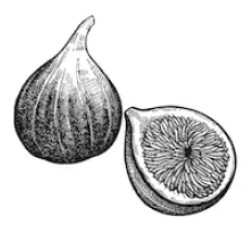
\includegraphics[width=1in,height=1.25in,clip,keepaspectratio]{fig1}}]{Michael Shell}
Use $\backslash${\tt{begin\{IEEEbiography\}}} and then for the 1st argument use $\backslash${\tt{includegraphics}} to declare and link the author photo.
Use the author name as the 3rd argument followed by the biography text.
\end{IEEEbiography}

\vspace{11pt}

\bf{If you will not include a photo:}\vspace{-33pt}
\begin{IEEEbiographynophoto}{John Doe}
Use $\backslash${\tt{begin\{IEEEbiographynophoto\}}} and the author name as the argument followed by the biography text.
\end{IEEEbiographynophoto}




\vfill




\end{document}
